\subsubsection{Aktualizacja systemu}
\begin{wrapfigure}{R}{0.1\textwidth}
	
\includegraphics[width=\linewidth]{images/pierwsze_uruchomienie_aktualizacja1.png}
\end{wrapfigure}

Kliknij na ikonę Dash 
\includegraphics[scale=0.35]{images/ikony_dash.png} i wpisz "Aktualizacje". W czasie wpisywania na ekranie wyników będą się pojawiały propozycje. Z wiersza "Programy" wybierz "Aktualizacje oprogramowania".

System sprawdzi, czy dostępne są aktualizacje dla twojego Ubuntu i wyświetli podsumowanie.

\begin{center}
	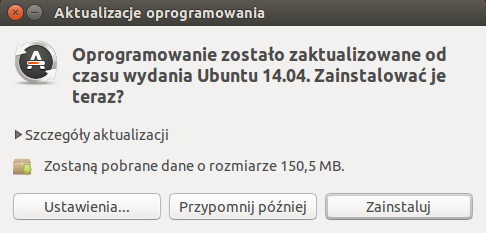
\includegraphics{images/pierwsze_uruchomienie_aktualizacja2.png}
\end{center}

Kliknij na przycisk \textbf{Zainstaluj} aby zainstalować aktualizacje. Zostaniesz poproszony o podanie hasła w celu uwierzytelnienia. Każda operacja mająca wpływ na cały system wymaga potwierdzenia. Zapobiega to przypadkowemu uszkodzeniu systemu.
\begin{center}
	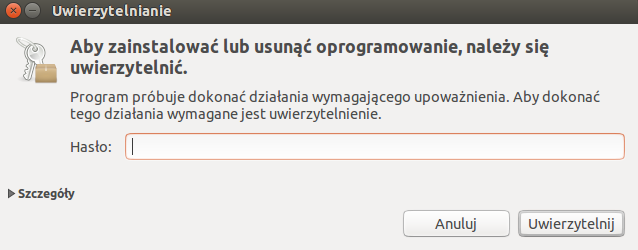
\includegraphics{images/unity_uwierzytelnienie.png}
\end{center}

Wpisz swoje hasło i potwierdź klawiszem Enter, lub kliknij na przycisk \textbf{Uwierzytelnij}. Teraz rozpocznie się proces pobierania i instalacji aktualizacji. Proces ten może potrwać od kilkunastu sekund do kilku minut, w zależności od tego jak dawno system nie był aktualizowany.

Kiedy aktualizacja się zakończy możesz zostać poproszony o zrestartowanie komputera. Restart jest potrzebny tylko jeżeli aktualizowane było jądro systemu lub sterowniki. Inne aktualizacje nie wymagają restartu komputera a jedynie restart zaktualizowanego programu.

W przyszłości system będzie automatycznie sprawdzał czy dostępne są aktualizacje i powiadomi cię o tym.
\clearpage
\subsubsection{Instalacja spolszczenia}
Jeżeli w trakcie instalacji systemu nie wybrałeś języka Polskiego lub nie miałeś połączenia z internetem aby ściągnąć potrzebne paczki językowe to tutaj dowiesz się jak zainstalować odpowiednie oprogramowanie.

Kliknij na ikonę Dash 
\includegraphics[scale=0.35]{images/ikony_dash.png} i wpisz "Języki". System sprawdzi stan spolszczenia systemu i zaproponuje instalację dodatkowych paczek. Jeżeli się na to zgodzisz to zostaniesz poproszony o potwierdzenie. Wpisz swoje hasło i potwierdź klawiszem Enter, lub kliknij na przycisk \textbf{Uwierzytelnij}.

W przyszłości aplikacja "Języki" pozwoli ci w łatwy sposób zmienić język systemu na każdy z wspieranych przez społeczność Ubuntu.
\clearpage
\subsubsection{Instalacja dodatkowych sterowników}
Prawdopodobnie nie wszystkie sterowniki zostały włączone podczas instalacji Ubuntu. Aby się upewnić, że sprzet jest prawidłowo obsługiwany Kliknij na ikonę Dash 
\includegraphics[scale=0.35]{images/ikony_dash.png} i wpisz "Sterowniki". Z wyświetlonych wyników wybierz "Aktualizacje i sterowniki. W otwartym oknie przejdź na zakładkę "Dodatkowe sterowniki". Poczekaj chwilę aż system zbierze dane o twoim komputerze i porówna je z bazą danych sterowników. Z wybranej listy będziesz mógł wybrać, który sterownik powinien zostac użyty.

Zmiana sterownika wymaga potwierdzenia. Wpisz swoje hasło i potwierdź klawiszem Enter, lub kliknij na przycisk \textbf{Uwierzytelnij}.

Więcej o wyborze sterownika przeczytasz w rozdziale \ref{sterowniki}: Sterowniki
\clearpage
\subsubsection{Instalacja dodatków}
Na koniec warto zainstalować kilka pakietów oprogramowania Kliknij na ikonę Dash 
\includegraphics[scale=0.35]{images/ikony_dash.png} i wpisz "Centrum Oprogramowania". Z wiersza "Programy" wybierz "Centrum oprogramowania". W prawym górnym rogu nowootwartego okna masz wyszukiwarkę. Wpisz w nią "restricted-extracts" i wciśnij enter. Poczekaj aż odnaleziona zostanie ta paczka. Z listy wybiuerz "Ubuntu restricted extracts". Najedź na nią i wybierz "Zainstaluj". Instalacja oprogramowania wymaga uwierzytelnienia. Wpisz swoje hasło i potwierdź klawiszem Enter, lub kliknij na przycisk \textbf{Uwierzytelnij}.

Paczka "ubuntu restricted Extras" zawiera w sobie
\clearpage